% !TEX encoding = UTF-8 Unicode

\documentclass[a4paper]{article}

\usepackage{color}
\usepackage{url}
\usepackage[utf8]{inputenc}
\usepackage{graphicx}

\usepackage[english,serbian]{babel}

\usepackage[unicode]{hyperref}
\hypersetup{colorlinks,citecolor=green,filecolor=green,linkcolor=blue,urlcolor=blue}

\usepackage{listings}
\definecolor{codegreen}{rgb}{0,0.6,0}
\definecolor{codegray}{rgb}{0.5,0.5,0.5}
\definecolor{codeblue}{rgb}{0.0,0,0.82}
\lstdefinestyle{mystyle}{
    commentstyle=\color{codegreen},
    keywordstyle=\color{codeblue},
    numberstyle=\tiny\color{codegray},
    stringstyle=\color{codegreen},
    basicstyle=\footnotesize,
    breakatwhitespace=false,
    breaklines=true,
    captionpos=b,
    keepspaces=true,
    showspaces=false,
    showstringspaces=false,
    showtabs=false,
    tabsize=4
}
\lstset{style=mystyle}

\usepackage[font=scriptsize,labelfont=bf]{caption}


\begin{document}

\title{Sinteza programa\\ \small{Seminarski rad u okviru kursa\\Metodologija stručnog i naučnog rada\\ Matematički fakultet}}

\author{ \href{mailto:anja.ivanisevic95@gmail.com}{Anja Ivanišević}, \href{mailto:mi14031@matf.bg.ac.rs}{Ivan Ristović}, \href{mailto:mi14042@matf.bg.ac.rs}{Milana Kovačević}, \href{mailto:vesna.katanic@gmail.com}{Vesna Katanić}}
\date{april 2018.}
\maketitle

\abstract

U ovom radu je prikazana sinteza programa kao savremena oblast računarstva. Sinteza programa je oblast koja se bavi automatskim generisanjem programa. Korisnik na neki način opiše željeni program, a zadatak sintezera je da ga generiše tako da on zadovoljava zadata ograničenja. Sintezer može svom zadatku da pristupi na različite načine, a neki od tih načina su detaljnije opisani u radu. Primene sinteze programa su brojne, od priprema podataka, popravka i dobijanja sugestija prilikom kodiranja do predloga mogućih optimizacija. Kao jedan od značajnijih pristupa sintezi, detaljno je opisana tehnika CEGIS. To je pristup sintezi koji u svojoj osnovi sadrži iterativno generisanje kandidata za traženi program i proveru da li taj kandidat zadovoljava date uslove. Ukoliko ih zadovoljava, on se prosleđuje korisniku kao krajnje rešenje.


\setcounter{tocdepth}{1}
\tableofcontents

\newpage

\section{Uvod}
\label{sec:uvod}

Danas skoro da ne postoji osoba koja nema pristup modernim tehnologijama. Potražnja za softverom je sve veca, a samo mali procenat ljudi ima adekvatna
znanja za njegovo programiranje. Standardni način programiranja se sastoji od dizajniranja algoritma koji rešava problem i njegove implementacije. Automatska sinteza programa ima potencijal da promeni generalni pristup implementacije programa. Ovakav način kreiranja softvera bi mogao da omogući i manje stručnim licima da programiraju bez dugokog poznavanja algoritama, struktura podataka i optimizacija.
Ideja je da korisnici daju opis željenih funkcionalnosti programu za automatsko generisanje koda (u daljem tekstu \emph{sintezeru}), a on će im automatski generisati neophodnu implementaciju.

Poslednjih nekoliko decenija došlo je do značajnog pomaka u razvoju automatskog rezonovanja, naročito u unapređivanju SAT (eng. \emph{Propositional satisfiability problem}) i SMT (eng. \emph{Satisfiability modulo theories}) rešavača \cite{SMT}, koji su sad u mogućnosti da reše i neke industrijske probleme \cite{PSE}. Ovaj napredak u automatskom rezonovanju dao je vetar u leđa razvoju programske sinteze koja svoja rešenja zasniva na logici prvog i drugog reda i automatskom dokazivanju teorema.

U ovom radu osvrnućemo se na neke primene programske sinteze, najveće izazove koji se u njoj javljaju, i neke tehnike zasnovane na CEGIS-u (eng. \emph{Counterexample-guided inductive synthesis}) koje su podstakle razvoj novih alata u ovoj oblasti.

\section{Primene}
\label{sec:primene}


Ovde pišem tekst.
Ovde pišem tekst.
Ovde pišem tekst.
Ovde pišem tekst.
Ovde pišem tekst.
Ovde pišem tekst.
Ovde pišem tekst.
Ovde pišem tekst.

\section{Izazovi}
\label{sec:Izazovi}

Pisanje programa koji može da sintetiše drugi program predstavlja veliki izazov. Naime, ovaj problem se može razložiti na dva potproblema:

\begin{itemize}
  \item Definisanje specifikacija željenog programa,
  \item Pretraživanje prostora mogućih programa u potrazi za onim koji zadovoljava definisane specifikacije.
\end{itemize}

Prostor programa se povećava eksponencijalno brzo u odnosu na veličinu željenog programa. Zbog toga postoje različiti pristupi njegovog pretraživanja, a neke od tih tehnika su opisane u poglavlju \ref{subsec:ProstorPrograma}. 

\subsection{Definisanje specifikacija}
\label{subsec:DefinisanjeSpecifikacija}

Generisani program treba da se ponaša na način koji to korisnik definiše. Međutim, precizno definisanje zahteva je zapravo mnogo teže nego što izleda na prvi pogled. Postoje različiti načini na koje se to može program može opisati. Može se opisati formalnim logičkim izrazima, kao i neformalnim metodama ili primerima ulaza i izlaza programa.

Formalno definisanje zahteva može često da izgleda komplikovano (možda čak i da deluje komplikovanije neko pisanje samog programa). Nasuprot tome, neformalne metode su mnogo prirodnije korisniku, ali dovode do drugih problema. Na primer, neka se željeni program definiše na osnovu primera njegovog ulaza i izlaza na sledeći način: \emph{“John Smith” -> “Smith, J.”}. Ovaj program vrši nama intuitivnu transformaciju niski, ali, na primer, da bi se on automatski generisao korišćenjem FlashFill \cite{FlashFill} programa, tj. program treba da pretraži prostor koji sadrži milione mogućih rešenja. Problem je u tome što programi nemaju ljudsku intuiciju, već se preprilagođavaju datim primerima ulaza i izlaza.

Većina programa koji se danas koriste su previše komplikovani da bi se u potpunosti opisali bilo formalnim bilo neformalnim metodama. Čak i ako bi se to nekako uspelo, opis programa bi mogao da bude toliko obiman kao i sama implementacija programa. Kako bi senteza ovakvih, realnih programa bila moguća, potrebno je omogućiti korisniku da na početku definiše željeni program do neke tačke, a da kasnije tokom sinteze, interaktivno sa računarom, postepeno dolazi do rešenja.

Upravo ovakvu napradnu pretragu koristi gore spomenuti program FlashFill. Tokom pretrage, on uključuje dodatnu komunikaciju sa korisnikom. Ovako on usmerava pretragu, te na kraju ipak uspeva da nađe rešenje u realnom vremenu.


\subsection{Prostor programa}
\label{subsec:ProstorPrograma}

Svaka uspešna sinteza programa vrši neki vid pretrage prostora mogućih programa (eng. \emph{search space}). Ovo je težak kombinatorni problem. Broj mogućih rešenja raste eksponencijalno sa veličinom programa, te pretraga svih kandidata nije moguća u realnom vremenu. Potrebno je pažljivo vršiti odsecanja dela prostora pretrage kako bi se došlo do rešenja u realnom vremenu.

Tehnike pretrage se mogu zasnivati na enumerativnoj pretrazi, dedukciji, tehnikama sa ograničenjima, statističkim tehnikama, kao i na kombinaciji nekih od nih.


\subsubsection{Enumerativna pretraga}
\label{subsubsec:Enumerative}

Tehnike enumerativne pretrage za sintezu prigrana su se pokazale kao jedne od najefikasnijih tehnika za generisanje malih programa. Razlog ove efikasnosti je u pametnim tehnikama \emph{čišćenja} (eng. \emph{pruning}) u prostoru programa koji se pretražuje. Glavna ideja je da se prvo na neki način opiše prostor pretrage u kome se nalazi žejleni program. To može da se postigne korišćenjem meta-podataka kao što su veličina programa ili njegova složenost. Kada se mogući programi numerišu po osobinama, mogu da se odmah odbace oni koji ne zadovoljavaju prethodno definisane specifikacije.

Kako na osnovu pretpostavki vrši velika odsecanja, može da se dođe do toga da pogrešno numeriše neki od programa i time izgubi neka od mogućih rešenja. Zato je enumerativna tehnika polu-odlučiva, ali u opštem slučaju je upotrebljiva i daje dobre rezultate i to relativno brzo.



\subsubsection{Deduktivna pretraga}
\label{subsubsec:Deductive}

Deduktivna sinteza programa je tradicionalni pogled na sintezu programa. Ovakvi pristupi pretpostavljaju da postoji celokupna formalna specifikacija željenog programa. Ovo je vrlo jaka pretpostavka imajući u vidu da ta specifikacija može da bude veoma velika ukoliko je program kompleksan. Rešenje se sintetiše postupkom dokazivanja teorema, logičkim zaključivanjem i razrešavanjem ograničenja.

Deduktivna pretraga je pretraga odozgo - na dole. Koristi tehniku podeli-pa-vladaj (eng. \emph{divide-and-conquer}). Program sintetiše tako što se prvo podeli na potprobleme tako da svaki od njih ima svoju specifikaciju. Rekurzivno se obrade potproblemi, a zatim iskombinuju podrešenja kako bi se dobilo glavno rešenje.

Deljenje problema na potprobleme koji mogu da se sintetišu odvojeno nije moguće u opštem slučaju. Ovo zavisi od prirode problema. U tom slučaju se deduktivna pretraga može iskombinovati sa enumerativnom. Kada deduktivna pretraga više ne može da razloži problem, enumerativnom pretragom (koja je odozdo - na gore) tda treba pretražiti prostor rešenja potproblema, i nakon toga spojiti dobijene rezultate.


If the underlying grammar allows for a rich set of constants,
the bottom-up enumerative search can get lost in simply guessing the
right constants. On the other hand, the top-down deductive technique
can deduce constants based on the accumulated constraints as the last
step in the search process.


\subsubsection{Tehnike sa ograničenjima}
\label{subsubsec:ConstraintSolving}

Mnoge uspešne tehnike sinteze programa u svojoj osnovi sadrže tehnike prilagođavanja datim ograničenjima (eng. \emph{constraint solving}). One se sastoje od dva velika koraka:
\begin{itemize}
  \item \emph{Generisanje ograničenja} - U opštem slučaju, kada se kaže prilagođavanje ograničenjima misli se na na pronalaženje modela za formulu koja opisuje željeni program. Osnovna ideja je da se specifikacija programa kao i njegova dodatna ograničenja zapišu u jednoj logičkoj formuli. Uglavnom se tom prilikom u formulu dodaju pretpostavke o rešenju.
  \item \emph{Razrešavanje ograničenja} - Formula u kojoj su zapisana ograničenja često sadrži kvatifikatore i nepoznate drugog reda. Ova formula se prvo transformiše u oblik pogodan za nekog od rešavača, na primer SAT ili SMT rešavač. Na ovaj način se problem pretrage svodi na problem ispitivanja zadovoljivosti prosleđene formule. Svaki nađeni model za tu formulu predstavlja jedno moguće rešenje koje zadovoljava data ograničenja.
\end{itemize}

TODO: primer?
We illustrate this idea on a simple example. Consider a small DSL
of bitwise operations upon a 8-bit input variable x:
...

\subsubsection{Statistička pretraga}
\label{subsubsec:Statistical}

Postoji veliki broj statističkih metoda koje mogu da se upotrebe za pretragu. Neke od njih su:
\begin{itemize}
  \item \emph{Mašinskog učenje} - Tehnike mašinskog učenja mogu doprineti ostalim pretragama uvodeći verovatnoću u čvorove granjanja prilikom pretrage. Vrednosti verovatnoće se uglavnom generišu pre sinteze programa: tokom treninga ili na primer na osnovu datih primera ulaza i izlaza. 

  \item \emph{Genetičkog programiranje} - Genetičko programiranje je metod inspirisan biološtkom evolucijom. Sastoji se od održavanja populacije programa, njihovog ukrštanja i mogučih mutacija. Svaka jedinka populacije se ispituje u kojoj meri zadovoljava specifikacije žejlenog programa. One jedinke koje bolje odgovaraju rešenju nastavljaju da evoluiraju. Uspeh genetičkog programiranja zavisi od funkcije zadovoljivosti.

  \item \emph{MCMC sampling} - MCMC sampling has been used to search for a desired program
starting from a given candidate. The success crucially depends on
defining a smooth cost metric for Boolean constraints. STOKE [124], a
superoptimization tool, uses Hamming distance to measure closeness
of generated bit-values to the target on a representative test input set,
and rewards generation of (almost) correct values in incorrect locations.


  \item \emph{Probabilistic inference} - Probabilistic inference has been used to evolve a given program by
making local changes, one at a time. This relies on modeling a program
as a graph of instructions and states, connected by constraint nodes.
Each constraint node establishes the semantics of some instruction by
relating the instruction with the state immediately before the instruction
and the state immediately after the instruction [45]. Belief propagation
has been used to synthesize imperative program fragments that execute
polynomial computations and list manipulations [62].

\end{itemize}

\section{CEGIS}
\label{sec:cegis}


\subsection{Motivacija}
\label{subsec:Motivacija}

Program se može sintetisati tako što se definišu njegove specifikacije i zapišu u vidu formule koja se prosledi SMT rešavaču (npr. Z3 [?]). SMT nađe valuaciju koja je zadovoljiva i to predstavlja rešenje. Problem nastaje u tome što formula koja se prosleđuje rešavaču sadrži univerzalne kvantifikatore koje usporavaju pretragu. Naime, rešavač bi u svakom slučaju pronašao rešenje za datu formulu, ali kako bi se to desilo u realnom vremenu, CEGIS (\emph{Counter-Example Guided Inductive Synthesis}) u sebi sadrži posebne tehnike za optimizaciju.

Za većinu realnih problema nije neophodno da se razmatraju svi ulazi i izlazi kako bi se došlo do programa koji radi tačno za svaki od njih. Ovako razmišljajući, problem se menja i postaje: \emph{"koji je najmanji podskup ulaza koji je potrebno razmatrati da bi se sintetisao program koji zadovoljava date specifikacije?"}.

CEGIS upravo traga za tim minimalnim skupom. U petlji, korišćenjem SMT rešavača, on postepeno dolazi do svih mogućih implementacija že\-lje\-nog programa koristeći sve ulaze koji su razmatrani do tog trenutka (počinje sa 0 ulaza). U sledećoj iteraciji on razmatra dalje. Paralelno sa tim, drugim SMT rešavačem pronalazi kontra-primer koji pokazuje da poslednji sintetisani program nije rešenje. Ukoliko kontra-primer ne postoji, poslednji sintetisani prigram je rešenje. Ukoliko se prođe kroz sve iteracije i ne pronađe se rešenje, specifikacija programa nije smislena.

Jedna od mogućih implementacija se može naći na \cite{CEGISimpl}.


\subsection{Arhitektura}
\label{subsec:Arhitektura}

CEGIS se sastoji iz dve faze, induktivne sinteze i verifikacije. Na početku sintezeru dajemo specifikaciju željenog programa. U fazi sinteze pronalazi se program kandidat koji može da zadovolji specifikacije. Nakon toga se u fazi verifikacije proverava da li taj kandidat zaista zadovoljava specifikacije. Ako verifikator ne uspe da pronađe kontra primer znači da smo pronašli traženi program. U suprotnom, verifikator prosleđuje sintezeru informacije o kontra primeru, koje će mu pomoći prilikom daljeg traženja novog kandidata. Na slici \ref{fig:cegis} predstavljena je opšta arhitektura CEGIS-a.

Ovakav vid pretrage zove se pretraga vođena kontra primerima (eng. \emph{counterexample-guided}), zato što je povratna informacija sintezeru kontra primer koji se dodaje u specifikaciju programa.

\begin{figure}[t]
    \begin{center}
        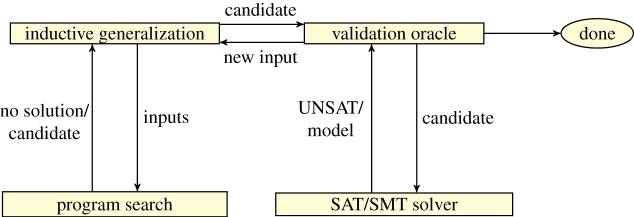
\includegraphics[scale=0.4]{resources/cegis.jpeg}
    \end{center}
    \caption{CEGIS petlja \cite{AboutPS}}
    \label{fig:cegis}
\end{figure}


Da bismo u potpunosti definisali CEGIS sintezu programa, potrebno je da odgovorimo na nekoliko važnih pitanja:

\begin{itemize}
    \item Kako treba da izgleda specifikacija traženog programa?
    \item Kako ćemo vršiti sintezu programa kandidata?
    \item Kako da proverimo da li program kandidat zadovoljava specifikacije?
    \item Kako da prosledimo povratne informacije za buduće kandidate?
\end{itemize}

\subsection{Primene CEGISa}
\label{subsec:PrimeneCEGISa}

U nastavku ćemo opisati kako se tri različite vrste sinteze programa koriste zajedno sa CEGIS idejom.


\subsubsection{Sinteza vođena oracle-om}
\label{subsec:OracleGuidedSynthesis}

Sinteza vođena oracle-om (eng. \emph{Oracle-guided synthesis}, u daljem tekstu \emph{OGS}) [?] pretpostavlja da imamo implementaciju programa koji želimo da sintetišemo, koja se naziva oracle program. Mi ćemo oracle tretirati kao crnu kutiju, možemo da joj damo ulazne vrednosti i dobijemo odgovarajući izlaz, ali nećemo razmatrati njenu implementaciju. Počinjemo sa skupom test primera, koji su parovi ulaz-izlaz. Pošto imamo oracle, možemo da kreiramo novi test primer jednostavno generišući random ulaze i od oracla ćemo dobiti odgovarajući izlaz za svaki prosleđeni ulaz. Oracle program će predstavljati specifikaciju za OGS.


\subsubsection{Faza sinteze}

OGS-u prosleđujemo biblioteku komponenti na osnovu koje sanitaizer kreira program koji je kandidat za rešenje. Faza sinteze će uzeti sve komponente i odlučiti kako da poveže njihove ulaze i izlaze tako da formiraju program. Ovako dobijem program će biti u SSA formi (eng. \emph{Static Single Assignment form} SSA) [?].

Na primer neka imamo biblioteku od tri komponente - dva sabiranja i jedno korenovanje. Njih je moguće povezati na sledeći način:

\begin{lstlisting}
program(x,y):
	o1 = add(x, y)
	o2 = add(o1, y)
	o3 = sqrt(o1)
	return o3
\end{lstlisting}

Primetimo da SSA forma jednostavno povezuje komponente me\-đu\-so\-bno, tako da ako želimo da imamo dva sabiranja moramo da obezbedimo dve komponente za sabiranje. Takođe primetimo da se vrednost $o2$ ne koristi, takozvani \emph{mrtvi kod}. U ovom slučaju to je poželjna karakteristika, jer ne moramo unapred tačno da odredimo koliko ćemo imati kojih operacija, već možemo samo da zadamo gornju granicu, a sanitaizer će generistai mrtvi kod za komponente koje se ne koriste.

Sanitaizer koristi test primere da ograniči broj načina na koje se komponente mogu povezati. On koristi SMT rešavač da odredi koje komponente da poveže kako bi program bio tačan za sve test primere. Ako SMT rešavač ne uspe da nađe rešenje, onda nijedan program koji koristi samo date komponente ne može da zadovolji sve test primere - komponente nisu dovoljne. U suprotnom vraća program u SSA formi koji zadovoljava sve test primere.


\subsubsection{Faza verifikacije}

Ako postoji rešenje mi program koji je kandidat za rešenje prosleđujemo fazi verifikacije. Ovaj korak koristi SMT rešavač da odgovori na sledeće pitanje: Da li postoji program $P'$, različit od kandidata za rešenje $P$, koji takođe zadovoljava sve test primere, ali se na nekom ulazu z ralikuje od $P$?
Pojasnimo ovo deo po deo. Iz faze sinteze dobili smo program $P$ koji je kandidat za rešenje i zadovoljava sve test primere. Ono što tražimo od verifikatora ja novi ulaz $z$ i novi program $P'$, takvi da za ulaz $z$ programi $P$ i $P'$ daju različite izlaze. Program $P'$ takođe zadovoljava sve početne test primere.
Drugim rečima pitamo se da li postoji više od jednog programa koji mogu da zadovolje sve test primere? Ako postoji nismo završili.
U ovom trenutku ništa ne pitamo oracle program. Može da se desi i da program $P$ i $P'$ daju netačan izlaz za ulaz $z$, ali jedino što je u ovom trenutku važno za verifikator je da oni daju različit rezultat.

Primer evo kako radi za dva test primera i komponente koje smo koristili u prethodnom primeru.

\begin{figure}[t]
    \begin{center}
        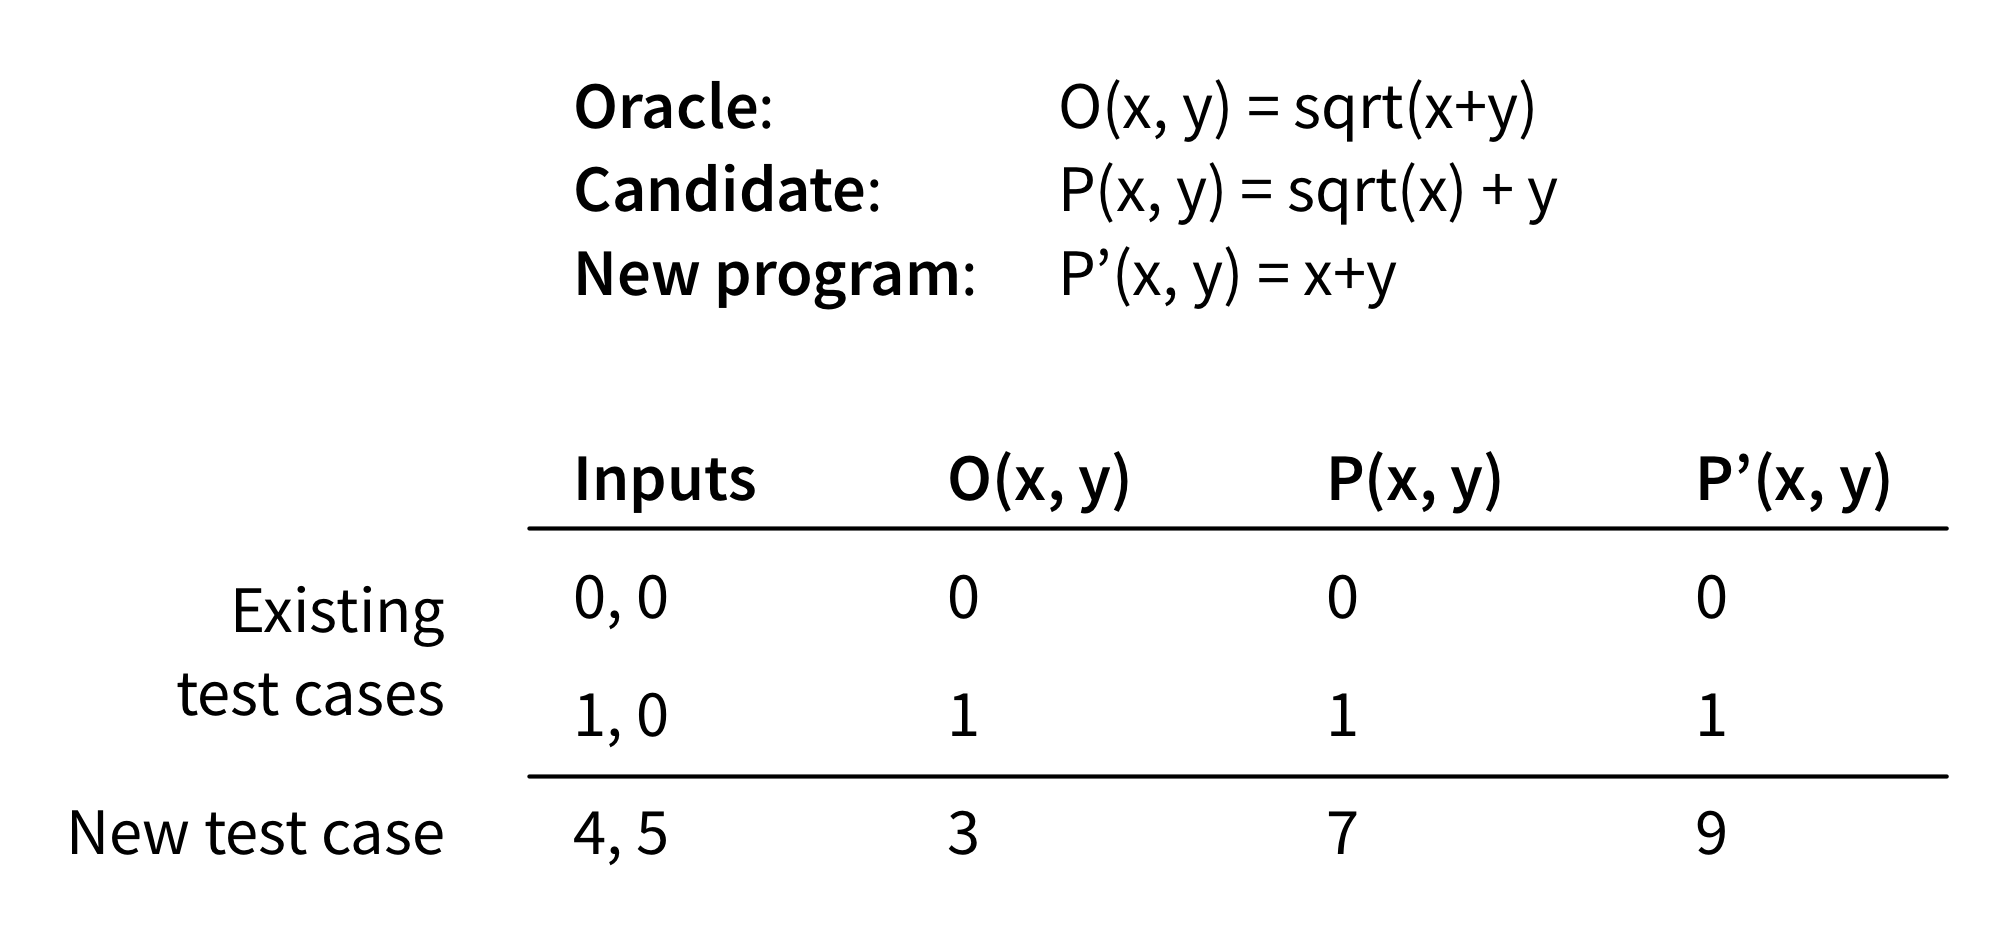
\includegraphics[scale=0.6]{resources/oracle-table.png}
    \end{center}
    \caption{Primer rada faze verifikacije}
    \label{fig:oraclePrimer1}
\end{figure}

U ovom slučaju imamo samo dva test primera $(0,0)$ i $(1,0)$. Sanitaizer nam daje program $P=\sqrt{x}+y$ koji je kandidat i koji zadovoljava oba test primera. Od verifikatora tražimo da nam da dve stvari: novi program $P'$ i novi ulaz $z$. U ovom slučaju on to i uspeva. Vraća novi program $x+y$ i novi test primer $(4,5)$. Na novom test primeru program $P$ i $P'$ daju različite izlaze: $\sqrt{4}+5=7$ dok je $4+5=9$. U ovom slučaju ispostavlja se da oba programa daju pogrešan rezultat sobzirom da je izlaz koji daje oracle $\sqrt{4+5}=3$. Međutim činjenica da se $P$ i $P'$ razlikuju nam je dovoljna da se u petlji vratimo nazad pomoću povratnog koraka.


\subsubsection{Povratni korak}

Ovaj korak razmatra novodobijeni ulaz $z$. Ulaz $z$ se daje oraclu i od oracla se dobija ispravan izlaz $z'$. Zatim se ulaz $z$ i $z'$ dodaju u skup test primera i ponovo prolazi kroz petlju.

Da bi smo bili u potpunosti sigurni u naše rešenje moramo da imamo i neku vrstu validacije. Problem je da tokom prolaska kroz CEGIS petlju možemo da nađemo jedinstveni program koji zadovoljava sve test primere pre nego što nađemo test primer koji taj program ne zadovoljava. Faza validacije treba da nakon završetka petlje potvrdi da program zadovoljava sve ulaze, a ne samo test primere.


\subsubsection{Stohastička superoptimizacija}
\label{subsec:StohastickaSuperoptimizacija}

Stohastička superoptimizacija pretražuje prostor programa i traži novi koji se ponaša isto kao i originalni, ali je brži ili efikasniji. Ovde ćemo takođe prtpostaviti da imamo implementaciju programa kao specifikaciju. Ovo nam neće predstavljati problem, jer tražimo optimalan skup instrukcija za dati kod.


\subsubsection{Faza sinteze}


Faza sinteze na osnovu tekućeg programa $P$ sintetiše novi program $P'$ primenom \emph{MCMC} (eng. \emph{Markov-chain Monte Carlo sampling}). Definiše se i \emph{funkcija prilagođenosti} (eng. \emph{cost function}) koja određuje koliko je program $P'$ blizu traženom programu i koliko je brz program $P'$ kako bi odredili da li da prihvatimo program $P'$ ili ne. Što je kandidat bliži željenom programu veće su šanse da bude prihvaćen, ali čak i progami koji su dalji ili sporiji od traženog mogu biti prihvaćeni sa nekom verovatnoćom. Ako je kandidat prihvaćen prelazimo na fazu verifikacije, a u suprotnom ponavljamo proces.


\subsubsection{Faza verifikacije}


U ovoj fazi se kandidat i ciljni program prosleđuju verifikatoru kako bi se utvrdilo da li su ekvivalentni. Pošto verifikator može da bude veoma spor pre prosleđivanja programa verifikatoru koriste se test primeri iz funkcije prilagpđenosti. Ako bilo koji od test primera ne uspe, sa sigurnošću možemo reći da kandidat ne može da bude ispravno rešenje pa se ni ne poziva verifikator.


\subsubsection{Povratni korak}

U ovoj fazi poredimo prethodno prihvaćeni program $P$ i novog kandidata $P'$. Ako je $P'$ bolji od $P$ onda ćemo nadalje njega razmatrati. Ako $P'$ nije bolji od $P$ verovatnoća da ćemo razmatrati $P'$ zavisi od toga koliko su programi $P$ i $P'$ slični.


\subsubsection{Enumerativna pretraga}
\label{subsec:EnumerativnaPretragaCegis}

Ovde ćemo za specifikaciju koristiti konačan skup test primera. Takođe pretpostavićemo da imamo gramatiku koja opisuje naš ciljani jezik. Na primer možemo uzeti gramatiku sa dve operacije \texttt{add} i \texttt{sub} i dve promenljive $x$ i $y$. \texttt{add(x, sub(x,y))} je jedan primer programa u ovoj gramatici.


\subsubsection{Faza sinteze}


Ideja enumerativne pretrage je da pretraži sve moguće programe. Programe delimo prema dubini, npr. program koji vraca $x$ ima dubinu $0$, a onaj koji vraća $x+y$ dubinu $1$.
Sintezu počinjemo od dubine $0$ i pritom numerišemo sve programe na ovoj dubini. Na dubini $k$, ispitujemo sve programe koji imaju oblik \texttt{operacija(a,b)}, gde su $a$ i $b$ bilo koji izraz dubine $k-1$. Broj programa koje treba ispitati ovakvim načinom pretrage raste eksponencijalno, pa se oslanjamo na povratni korak kako bi ubrzali pretragu.


\subsubsection{Faza verifikacije}


Pošto nam se specifikacija programa zasniva na test primerima u ovoj fazi ćemo jednostavno pokrenuti sve test primere i uporediti rezultate. Ako program daje odgovarajuće izlaze za sve test primere završili smo.


\subsubsection{Faza verifikacije}


Jedan od načina da smanjimo prostor pretrage je da na dubini $k$ ne razmatramo sve programe dužine $k-1$ već samo različite programe. Postavlja se pitanje kako da odredimo da li su dva programa različita? Pošto smo ciljni program definisali pomoću test primera nije bitno da li su nam dva programa semantički jednaka, već nam je bitno da za iste test primere daju različite rezultate. Na ovaj način smo iz pretrage izbacili mnogo programa koji nisu semantički jednaki, ali se isto ponašaju u našem slučaju.

\newpage
\section{Zaključak}
\label{sec:zakljucak}

Razvojem tehnika automatske sinteze programa postavlja se pitanje da li će programeri moći da prestanu da govore računarima \textbf{kako} da rade, već da se fokusiraju na to da im kažu \textbf{šta} treba da urade. Ova oblast još uvek nije dovoljno razvijena da bi se koristila za razvijanje realnih, velikih aplikacija. Potrebno je još rada da bi se došlo do toga. Najveći potencijal ima induktivna sinteza programa.
Iako teorijski deluje da ovaj pristup nije dovoljno efikasan, te da će se izvršavati predugo, CEGIS je, kao vodeći predstavnik ove grupe, u praksi pokazao neočekivano dobre rezultate. Uprkos tome, i uspešno sintetisanje manjih programa može značajno da olakša rad programerima. S obzirom na to da najveći deo vremena programeri provedu pišući manje delove koda, pa i automatska sinteza samo tih delova može značajno da ubrza njihov rad.


\addcontentsline{toc}{section}{Literatura}
\appendix
\bibliography{literatura}
\bibliographystyle{plain}

%\appendix
\section{Dodatak}
Ovde pišem dodatne stvari, ukoliko za time ima potrebe.
Ovde pišem dodatne stvari, ukoliko za time ima potrebe.
Ovde pišem dodatne stvari, ukoliko za time ima potrebe.
Ovde pišem dodatne stvari, ukoliko za time ima potrebe.
Ovde pišem dodatne stvari, ukoliko za time ima potrebe.


\end{document}
